\documentclass[12pt]{article}
\usepackage{amsmath}
\usepackage{subcaption}
\usepackage[utf8]{inputenc}
\usepackage{wrapfig}
\usepackage{float}
\usepackage{graphicx} % Required for inserting images
\usepackage{booktabs} % This and below for tables
\usepackage[breaklinks]{hyperref}
\hypersetup{colorlinks=true, linkcolor=Black, citecolor=Black, filecolor=Blue,
    urlcolor=Blue, unicode=true}
\usepackage[margin=1.2in]{geometry} % Adjust border

\renewcommand{\thesubsubsection}{(\alph{subsubsection})}

\begin{document}


\title{STA4026S Analytics - Neural Networks}

\author{Assignment 1\\
        Laurence Walton\\
        \href{mailto:wltlau003@myuct.ac.za}{wltlau003@myuct.ac.za}
}
\date{August, 2023}

\maketitle

\subsubsection{}
In the context of neural networks the soft-max activation function is used to turn an output layer into a probability distribution where each node has a value between 0 and 1 and the sum of the nodes is 1. This is relevant for multi-class classification problems because with soft-max applied each output node value can be treated as a probability where predictions may correspond to the node with the highest probability, and the error between the predicted probabilities and the true class labels can be used to adjust the network during the training process. The soft-max ensures that the predictions are scaled such that the error accurately reflects the disparities between the predicted probabilities.
The soft-max function in matrix form is:

\[
\sigma(z^n_j) = \frac{exp(z^n_j)}{\sum_{k=1}^q exp(z^n_k)}
\]

Where:
\begin{align*}
z^n_j & : \parbox[t]{0.7\textwidth}{The $j$-th node in the $n$-th training example, i.e. a value from the $q \times N$ output matrix where each row represents a node in the output layer and each column represents a training example} \\
\end{align*}

\subsubsection{}
A potential numerical pitfall in evaluating the cross-entropy error function arises if the predicted probability for a class is 0, as the evaluation would include the logarithm of 0 which is obviously undefined. This is mitigated by using activation functions such as the soft-max, where no predictions can be zero due to exponentiation. However, due to floating point imprecision in software, predictions could be rounded to zero in the soft-max, and therefore cause undefined behaviour in the cross-entropy error function.

\subsubsection{}

Plotting the cross-entropy error obtained on the validation data for varying values of $\nu$ yields the following curve, where I found the $\nu$ value of $0.09261443$ corresponds to the minimum error of $0.1259723$:

\begin{figure*}[!ht]
\centering
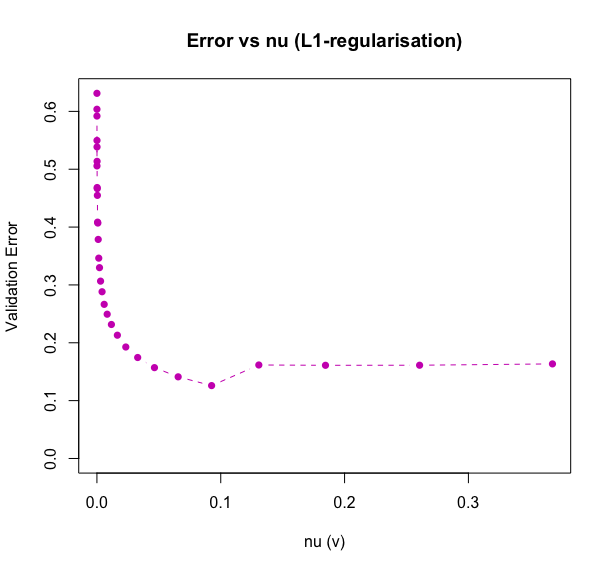
\includegraphics[width=0.8\textwidth]{question_c_plot.png}
\end{figure*}

\newpage
\subsubsection{}
Now I include use a new ANN which uses Rectified Linear Units (ReLU) as the hidden layer activation function. This is superimposed over the previous curve which showed an ANN using Tanh activation functions. I found the $\nu$ value of $0.09261443$ corresponds to the minimum error of $0.1207693$:

\begin{figure*}[!ht]
\centering
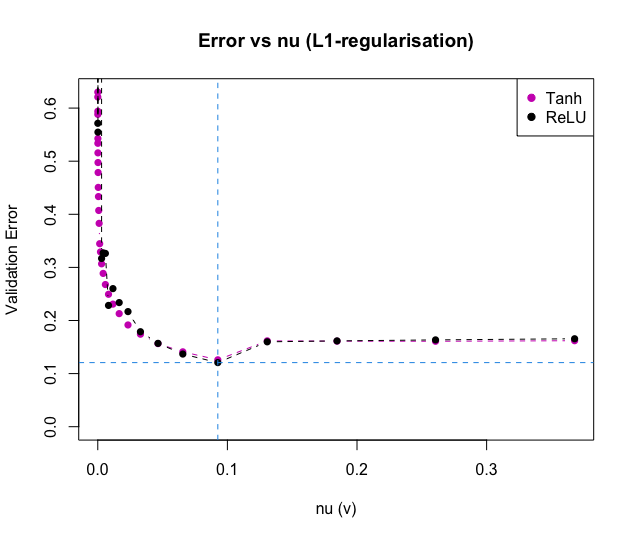
\includegraphics[width=0.8\textwidth]{question_d_plot.png}
\end{figure*}

\newpage

\subsubsection{}
Here I trained a neural network with tanh activation in the hidden layer on the complete data set, both with and without L1 regularization. Comparing the magnitude of the parameters between these two models provides insights into the model's complexity. L1 regularization introduces more 'sparsity', essentially reducing the effective number of parameters. In this case specifically, with L1 regularization, many of the model's parameters shrank to near-zero or zero and the largest parameter magnitudes were also reduced. The fact that the regularization promotes such strong sparsity indicates that the original model, without regularization, might have been overfitting the data, capturing excessive variance instead of the true underlying patterns. In simpler terms, the original model had high variance, which might have compromised its generalization capability on unseen data. The reduced number of effective parameters and reduced magnitudes show that the model can better perform on data outside of the training set.

 
\begin{figure*}[!ht]
\centering
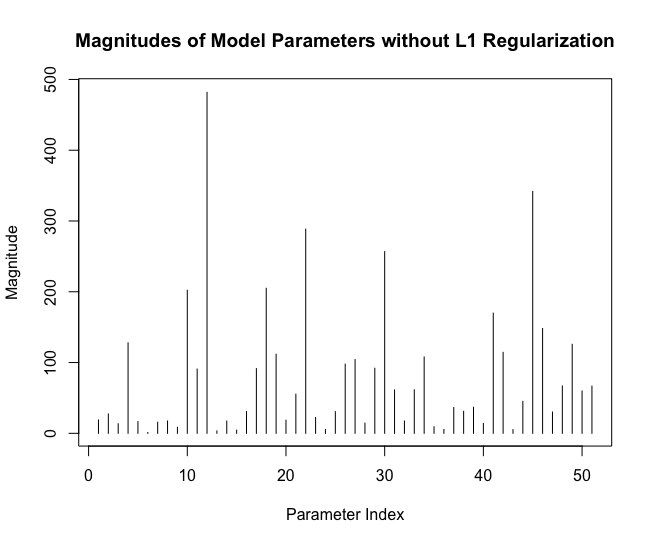
\includegraphics[width=0.5\textwidth]{question_e_plot_B.png}
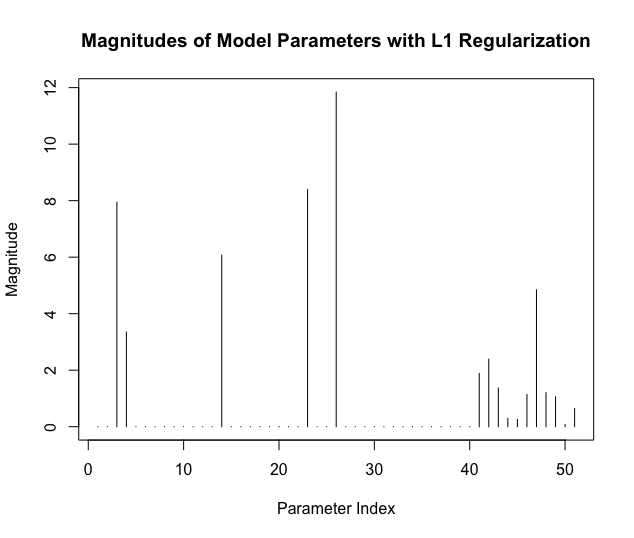
\includegraphics[width=0.5\textwidth]{question_e_plot_A.png}
\end{figure*}



\subsubsection{}
\begin{figure*}[!ht]
\centering
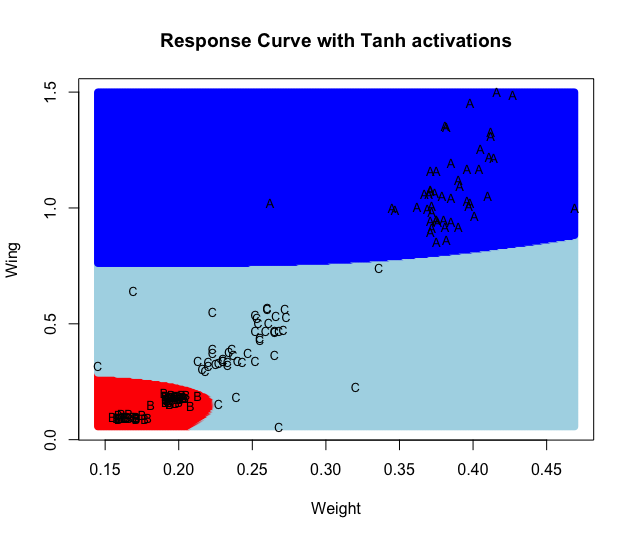
\includegraphics[width=0.7\textwidth]{question_f_plot_A.png}
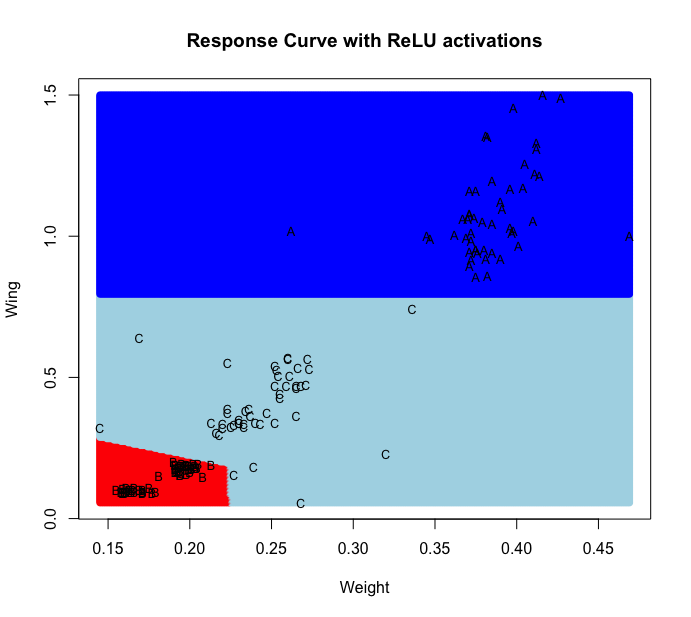
\includegraphics[width=0.7\textwidth]{question_f_plot_B.png}
\end{figure*}




\end{document}
